\documentclass[12pt,a4paper,openright,oneside]{book}

\input{thesis-setting.tex}

% 仅用于测试
\usepackage{blindtext}
\usepackage{algorithm}  
\usepackage{algorithmic} 
\floatname{algorithm}{算法}
\renewcommand{\algorithmicrequire}{\textbf{初始化}}   %改成后面的小标题
\renewcommand{\algorithmicensure}{\textbf{确认}} 
\renewcommand{\algorithmicif}{\textbf{如果}} 
\renewcommand{\algorithmicthen}{\textbf{然后}} 
\renewcommand{\algorithmicwhile}{\textbf{当}} 
\renewcommand{\algorithmicend}{\textbf{结束}} 
\renewcommand{\algorithmicelse}{\textbf{其他}}  

\title{\textsf{比如我举个例子}}
\author{{\kai 谁知道呢}}
\date{May 20, 20xx}

\begin{document}

\sloppy

\pagenumbering{Roman}

% 封皮
\frontmatter
\input{cover.tex}

\setcounter{page}{1}
\renewcommand{\baselinestretch}{1.25}

% 中文摘要
\renewcommand{\baselinestretch}{1.5}
\fontsize{12pt}{13pt}\selectfont


\chapter{摘~~~~要}
\markboth{中~文~摘~要}{中~文~摘~要}

..............

综上, 本文主要做的工作有
\vspace{-10pt}
\begin{enumerate}
	\item 分析 A
	\item 分析 B
	\item 提出 C
	\item 提出 D
	\item 提出 E
\end{enumerate}
\vspace{-10pt}

\vspace{1em}
\noindent {\fHei 关键词:} \quad 学位论文, 模板, \LaTeX

\clearpage
\endinput

% 英文摘要
\renewcommand{\baselinestretch}{1.5}
\fontsize{12pt}{13pt}\selectfont

\chapter[ABSTRACT(英文摘要)]{ABSTRACT}
\markboth{英~文~摘~要}{英~文~摘~要}
%\noindent 
The networking technology of mobile underwater acoustic sensor networks is one of the important reserch topics of underwater acoustic sensor networks(UWASN). Using acoustic wave as the propagation medium, underwater communicatione owned characteristics of high bit error rates and unreliability. Meanwhile, the high dynamic nature of the network topology brought by mobile nodes causes various challenges in the development and design of UWASN. For ocean resource exporlation and national marine security, it is a very important problem to develop the UWASN and its appilication.

The UWASN can be divided into three layers: network layer, data link layer, and physical layer. The data link layer plays a vital role in providing reliable links for upper-layer network protocols. It can be divided into logical link layer (LLC) and media access control layer (MAC). This paper focuses on the  media access control(MAC) protocols in the UWASN

After analyzing the classification and research status of the current MAC protocol for UWASN, the paper proposes a protocol for the use case of a single-hop UWASN in which mobile nodes collect data from multiple fixed nodes.
The protocol called PAMC-M for Mobile UWASN is playload adaptive and based on MACA and CSMA.Performance analysis and simulation verification show that the proposed protocol performs well compared with the traditional contention-based protocol UWALOHA and SFAMA.

\noindent The main results of the paper are as follows:
\vspace{-12pt}
\begin{enumerate} \setlength{\itemsep}{0pt}
	\item For the scenario where a small number of mobile nodes access a network composed of fixed nodes and collect data from fixde nodes, a mobile node access mechanism is designed. Mobile node periodically send broadcast frames(BCT) and fixed nodes execute corresponding processing according to the received frame. The design of the broadcast frame enables mobile nodes to access the network at a small cost.
	\item Considering unreliability of mobile UWASN, a data frame retransmission mechanism was proposed. Retransmiting data frame immediately instead of making handshake once again, will greatly improve the transmition efficiency. 
	\item The collision probability becomes larger with the network load increases.Thus, an adaptive load-adaptive data frame transmission mechanism is proposed. The data frame is transmitted once after one handshake in the low-load mode, twice in the high-load mode. Performance analysis and simulation show that the adaptive load-adaptive transmission mechanism makes the protocol perform well under different network loads, improving network throughput and reducing transmission delay.

\end{enumerate}
\vspace{-12pt}

\vspace{1em}
\noindent {\textbf{Key Words:}} \quad Underwater acoustic sensor network, Media access control, Competitive MAC protocol, Mobile node access, Load adaptivity

\clearpage
\endinput

\renewcommand{\baselinestretch}{1.25}
\fontsize{12pt}{12pt}\selectfont
\phantomsection
\addcontentsline{toc}{chapter}{\fHei 目录}
\tableofcontents


\mainmatter

\renewcommand{\baselinestretch}{1.0}

\sHalfXiaosi\fSong

% 正文内容
\chapter{绪论}
水声传感器网络(UnderWater Acoustic Sensor Networks, UWASN)指的是在一定的水下区域内,通过各种传感器获取信息,并对水下节点进行水声通信和组网,进而实现信息的传输目的/cite{Underwater acoustic sensor networks}。UWASN可用于海洋灾害预警预报,深海能源与资源开发,海洋环境监测,维护国家海洋安全等方面。


\section{研究背景}
UWASN由多个水下固定传感器节点和移动节点如UUV和AUV等组成,这些节点被布放在水下一个给定区域内,共同执行观测任务。下图是一个典型的水声传感器网络,AUV、固定结点和海面浮标之间可以相互通信,海面浮标和控制中心利用卫星通信。
\begin{figure}[ht]
	\centering
	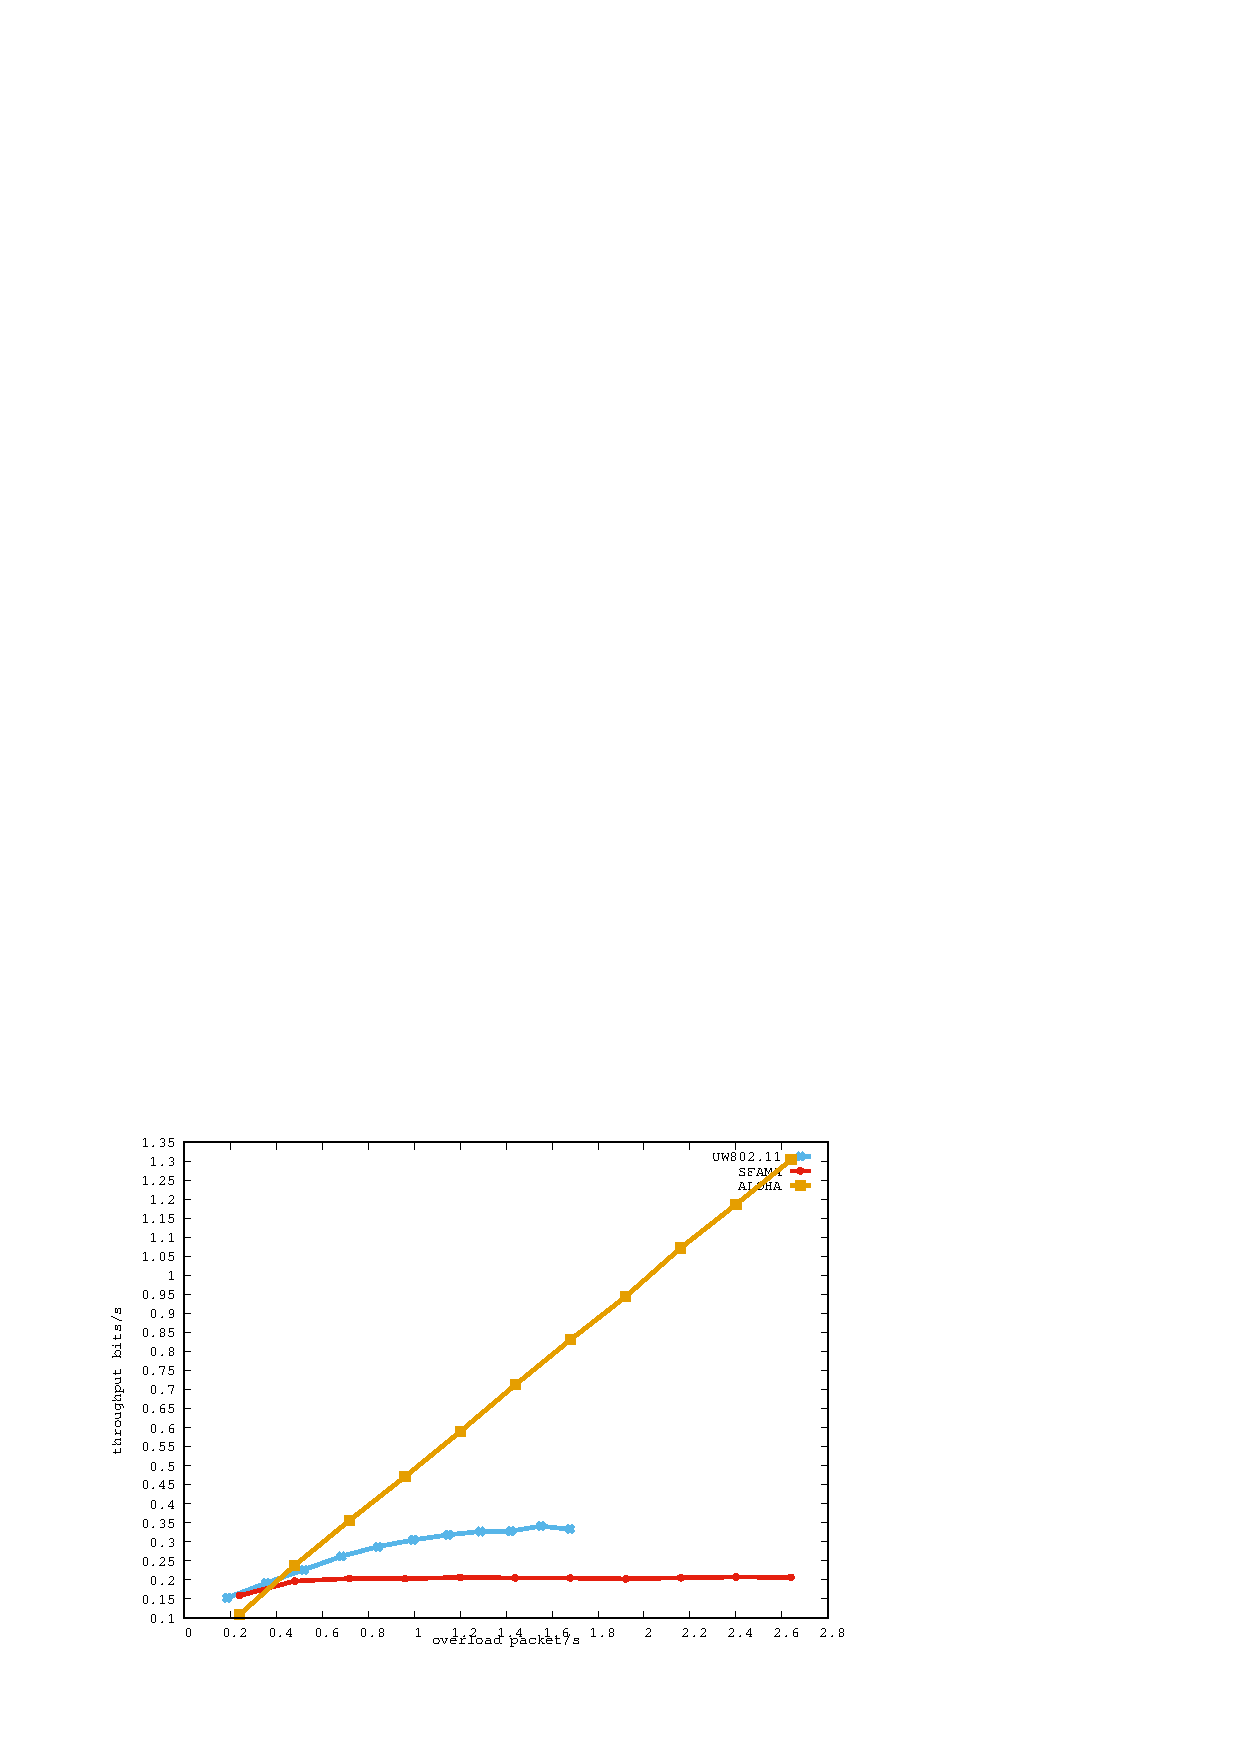
\includegraphics[scale=0.25]{figures/1.png}
	\caption{
		水声传感网络
	}
	\label{fig:example}
\end{figure}

其中,搭载有各种设备的AUV可以在水下按特定轨迹航行,是水下传感网络中常用的移动平台。AUV的加入为海洋立体观测提供了可能,扩大了网络的监控范围;同时AUV可以对网络进行配置,如节点失效时,AUV可以检测通信空洞并指导布放新节点,提高网络的稳健性。UWASN也可以为AUV的导航提供支持,进行水下定位等。

\subsection{水声传感网络发展过程}
美国是最早开始研究水声传感网络的国家。1994年,美国伍兹霍尔海洋研究所(WHOI)开发了第一代水声通信局域网(ALAN),该网络由一个海面浮标站和十几个1000m水深的海底节点构成,主要功能是将海底节点产生的数据发往水面站以及将水面站产生的控制信息发向海底节点。2005年WHOI用水声传感网络进行了海底地震探测实验。该网络由3个不同的水下传感器组成,每天向系在船上的浮标发送六次水声数据,这些浮标可通过卫星中继将数据转发到岸上。网络允许的最大上行传送速率是4kbps,每天可上传数据达1.4MB。

欧共体在MAST计划的支持下开展了一系列的水声通信网络研究,主要包括ACME,LOTUS、SWAN、ROBLINKS等子计划。其中ACME是研究基于浅水网络的稳健通信和网络协议,网络中节点最小数为3,水深6-10米,节点之间的距离是200-2000米,最高数据率是lkbit/s。LOTUS主要是研究基于超浅水域的长距离通信设备,其中点对点之间的通信距离可达到10km,载波频率为8kHz,最高数据速率4kbit/s,该系统针对超浅水域中存在的强时变的混响干扰以及多用户干扰等问题进行了技术攻关。使用三维水听器阵列进行空间分集,同时对每个发送端进行匹配,目前该系统已经进行了两次海上试验。SWAN计划的目标是在浅海条件下建立通信仿真模型.研究各种无训练条件下MEMU阵列处理方法。ROBLINKS计划主要是研究浅海条件下,水深20-30m,距离大于10km的稳健通信项目,开发新的最佳相关信号处理算法是其研究重点,通过连续信道辨识技术,提高通信系统对周围环境变化的适应能力,并对算法进行海上验证。

中国在水声传感网络领域的研究起步较晚。主要研究机构有中科院声学所、哈尔滨工程大学、浙江大学、东南大学、厦门大学、、中国海洋大学、西北工业大学等。研究内容主要是低速率远程通信和高速率近程通信,同步技术以及组网技术等。

\subsection{水声传感网络协议栈}
水声传感网络按分层结构一般可以分为物理层、数据链路层,网络层。
\paragraph{物理层}
物理层负责数据的调制解调,把数字信息转换成能在水声信道中传输的声信号。在接收端,检测被噪声及其他信道失真畸变的信号,并把信号恢复成原传送的数字信息。面临的挑战是如何克服水声信道的恶劣条件,长传播时延、高延时抖动、窄带宽、高误码率等特点对信息传输带来的影响,如何对长延时网络进行同步,以及如何简化设计发送端和接收端来降低成本提高性能。水声网络物理层主要的技术有相干解调、非相干解调、正交频分复用(Orthogonal Frequency Division Multiplexing,OFDM)和多输入多输入(Multiple Input Multiple Output,MIMO)技术。
\paragraph{数据链路层}
数据链路层负责将来自网络层的指令和数据封装成帧,帧是数据链路层固有的结构,它含有足够的控制信息,保证数据可以通过网络成功发送到目的节点。数据链路层还负责把从物理层接收到的二进制数据重新组装成帧。数据链路层协议面临的挑战是
如何使每个传感器节点都可以公平、有效分享带宽资源,使网络获得尽可能高的吞吐量,同时使占有时延尽可能小,消耗能量尽可能少。MAC协议应用在这一层中。
\paragraph{网络层}
网络层的任务是选择合适的路由信息,确定和分发源节点和目的节点之间的路由搜索及维护信息。要功能包括邻居发现、分组路由、拥塞控制和网络互联等功能。网络层面临的挑战是
如何使路由查找时间尽可能短,减少引入的额外时延,如何使维护路由的控制信息应尽量少,如何避免拥塞并提供QoS保证。



\subsection{面临的问题}
要达到可靠高效的端到端传输面临很多挑战,主要体现在以下几个方面:

(1)节水声信道可用带宽一般只有几kHz到几十 kHz,且随着通信距离的增加而减少,通信速率低。

(2)水声信道存在复杂的时、空、频变及强多途、高噪声、Doppler效应等因素,误码率高且中断概率大。

(3)声波传播速度低,传播时延长。

(4)节点移动性,由于水流等环境因素影响以及搭载平台的关系,大多数水下传感器节点存在着不同程度的移动,节点的移动导致传播时延变化。

(4)网络拓扑高动态:由于海洋环境恶劣,水下节点较容易出现故障或短暂失效,导致了网络节点不稳定的邻居关系。

(5)网络节点能量受限:水声节点长期工作在水下,充电困难且费用高,是能量资源严重受限的系统,节点之间相对更远的距离,以及为了弥补信道损耗,接收器对信号做了更复杂的处理都大大增加了能量的消耗。水声单位能量资源能传输的数据量比陆地无线通信低3个数量级。

水声网络大多是面向特定任务应用场景,以满足预定需求为设计目标,既可单独组网,也可与水下有线网络混合组网。预定任务的不同需求,如节点移动性、节点布署密度、网络覆盖范围、网络生命周期、网络传输可靠性等,将导致水声网络的不同设计。

\section{研究内容}
本研究针对有移动节点接入和水下固定传感器组成的小规模单跳网络,结合海洋信息采集中对移动水声传感网络的各类需求,从设计移动节点接入机制、降低整体传输时延等方面入手,进行了如下的研究:
\begin{itemize}
	\item 针对少量移动节点接入固定节点网络,单向采集固定节点数据的场景,设计移动节点的接入和离开机制。移动节点加入固定节点网络时,需要发送广播包通知固定节点进行数据传输,充分利用广播包特点,降低移动节点接入离开机制的开销,是流程设计时的重点。
	\item 针对移动水声网络的不可靠性高的特性的特性,设计数据帧重传机制。数据重传时从握手机制重新开始带来的时间和能耗开销太大,在第一次传输时给数据帧重传设计专有的机制是必要的。
	\item 针对网络负载较大时控制帧冲突概率较高的问题,设计自适应负载变化的数据帧发送机制。协议设计时,低负载网络和高负载网络的优化方向各不相同,因此能够自适应负载变化的协议可以更好得应对各种网络场景。
\end{itemize}

\section{章节安排}
本文的章节安排如下,

第一章绪论,主要介绍了水声传感网络的概念、发展历史和体系结构,说明了本文的研究背景和应用场景,提出了研究需要解决的问题,在此基础上引出了研究的主要内容。

第二章介绍了水声网络MAC协议的分类,分析了移动水声网络MAC协议研究的国内外现状。

第三章重点介绍了两个竞争型水声传感网络MAC协议,UWALOHA和SFAMA。

第四章针对有移动节点接入的单跳水声网络,提出了基于竞争的MAPA-CSMA协议。首先介绍了MACA和CSMA协议的基本原理。然后,重点介绍了移动节点的接入离开机制、数据帧重传机制和不同网络负载情况下的数据帧发送机制。

第五章介绍了提出的MAPA-CSMA协议的具体实现流程,并对协议性能进行了理论计算。

第六章介绍了仿真的工具NS2和平台Aqua-Sim,给出了四个性能指标,并分析了仿真实验的结果。

\endinput
\chapter{水声传感网络MAC协议研究现状 }
\section{水声传感网络MAC协议分类}
\begin{figure}[ht]
	\centering
	\includegraphics[scale=0.2]{figures/cha.png}
	\caption{
		水声传感网络
	}
	\label{fig:example}
\end{figure}
无线传感网络使用的MAC协议,通过信道占用方法可以分为竞争协议、非竞争协议和混合协议。竞争协议包括了ALOHA、载波侦听多址接入CSMA、基站捕获多址接入FAMA、冲突避免多址接入MACA等,非竞争协议包括了时分多址TDMA、码分多址CDMA、频分多址FDMA,混合协议包括了时空MAC(Spatial—Temporal MAC,ST-MAC)等。
\subsection{竞争协议}
基于Aloha的MAC协议有很多。纯A10ha协议非常简单:只要有节点想要发送数据,就立刻发送数据,无需考虑信道是否空闲。由于不侦听信道,会与正在发送中的数据包冲突,使得冲突节点发送的数据包被接收后都是无用的,而被丢弃。这种方式不仅降低了吞吐量,也浪费了能量。一个对纯Aloha改进MAC协议叫做Aloha—HD(Aloha谢tllHalfDu口lex,半双工A10ha协议)。Aloha-HD中,当节点意识到信道中的数据的目的节点是自己,该节点会一直保持接收数据模式,而不发送数据。如果信道中的数据不是发给自己,那么与纯A10ha一样,节点如果有数据发送可以立即发送。然而,Alolla一皿的前提条件是,能够接收到数据包的包头。Aloha另一个简单的变体是Aloha-CS(Aloha wi也CarrierSensillg,载波侦听Aloha协议)。Aloha.CS中要求只要信道中有数据,节点就不可以发送数据。然而,Aloha.cS不是侦听信道的状态,而是通过检测半双工的调制解调器是否在接收数据。Sl础ed.Aloha(时隙的Alolla)也被水下通
信考虑,即节点共享相同的同步时间,并且仅在时隙的开始时发送数据。然而在水下,
它的效率是低于在无线电中的效率。这是由于为了补偿不同的传输时延,需要长的保护
时间导致的。Nittllita Cllil.dchoo等人125J提出了Aloha的另外两个变种:Aloha.CA(Aloha
Notification,预知的Aloha协议)。这两个变体都利用节点从信道中收到的数据包,获
取数据包的发送端、接收端、以及发送端与接收端的时延,把侦听得到的信息添加到一
个数据库表中来避免冲突,以提高吞吐量。
载波监听多路访问(CSMA)代表了另一类的基于竞争的NoC协议。CsMA本身
要求数据包传输的时间应该远远大于传播延迟,然而在典型的水下网络是很难满足这个
条件的(由于水下大的延迟)。在水声传感器网络中直接使用CSMA会导致一个非常
长的漏洞时间。CS姒的另一形式在【26J中提出。在此,信道被侦听了一个很短的时间,
以避免一些必定产生冲突传输的模式。尽管可能是过于保守的行为【2‘71,其但性能良好。
冲突避免的CSMA(csMA.cA)也是一种选择。CSMA.CA以连接建立的更高的延迟
为代价减少冲突的机会。这是由于需要等待RTS/CTS交换的完成。水下带有数据包序
列的MACA在[28'29]中提出。DACAP(四)和APCAP【311就是CSMA—CA机制很好的例子。

然而,多跳拓扑结构可能导致控制包和数据包之间的碰撞。为解决这个问题,报文分片
【32】被提出。另一种方法是控制包单独使用一个信道【331。【34】进一步扩展,使用多信道进
行数据通信。时间槽的FAl、压A(Slo地d—FAMA)【35]是基于为陆地传感器网络设计的
FAMA【36l协议的改进。FAMA协议将时间分槽,载波侦听和握手技术结合在一起。
Slotted.FA讹~的主要原理与CSMA很相似,但Slotted.FAMA把时间划分成时间片,并
且要求节点只能在时间片的开始时发送数据包或者控制包如果一个节点想要发送数据
包,该节点必须等到下一时间片的开始,然后才能开始它的CSMA过程。Slo讹d.FAMA
基本上是融合了CsMA和Slo讹d-A10ha。为提高网络的性能,另一个想法就是重用。
R口T【3刀和DOST【381通过限制发送端而重用信道。MFAMA【39】允许发送者和多个接收者之
间发起多个会话。发送者利用偷听到的信息计算邻居节点之间的会话安排,以选择合适
的发送数据的时间。T.Lolli【15】是一个基于预留机制的竞争MAC协议。节点竞争信道的
使用权,然后发送数据。每个时间帧包含若干个争用回合(CR,Contention RouIld)和
一个无竞争的数据发送时间段。在竞争阶段,要求节点在CR时发送一个tone信息,然
后侦听信道来判断是否竞争成功。如果只有该节点竞争信道,那么该节点在接下来的数
据时间段(DP,Data Period)发送数据.如果多个节点在同一个CR竞争信道,那么每个
节点都会检测到竞争。然后这些竞争的节点会回退。在接下来的某个cR重新竞争信道。

\subsection{非竞争协议}
基于固定分配的MAC协议有频分多路复用、时分多路复用、码分多址复用。
频分多路复用(FDMA,Frequency
DiVision
Muhiple Access)把信道划分为若干个
子信道,然后把子信道分配给指定的节点使用。只有节点放弃使用子信道时,其他节点
才可以使用。虽然FDNo在陆地无线网络的性能很好,但由于水声信道的可用带宽窄,
如果把信道划分成小的子信道,传输信道的相干带宽可能大于子信道的带宽。相应的,
会造成使用不同子信道的节点的衰减[401。特别是,如果在数据量大的水声传感器网络中,
由于子信道是固定分配给节点的,不具有适应动态变化的网络环境的能力,因此,FDMA
的性能会低下14H21。
时分多路复用(II)MA,Time
Division
Multiple Access)是把时间划分为时间片而
分给节点的接入方法。一个时间片只分配给一个用户使用,每个节点只在给定的时间片
传送数据。在陆地网络中,有很多使用II)MA技术,如GSM(Global
[43】,Is 136
System
ofMobil姆)
m】。然而,TI)m为了避免节点之间分配的时间片有冲突,必须在时间片之
间加入一个短的时间片,即保护时间(guard time),这个开销比FDMA还要大【451。另
一个缺点是水下环境的长传输时延使得TDMA时间同步很难实现。因此会发生数据冲
突,降低系统性能。
与FDMA、TDMA不同,码分多址复用(CDMA,Code
DiVision
MmtiDle Access)
并不划分时间和带宽,而是允许所有节点同时在同一个信道上发送数据。通过给每个节
点分配不同的扩频码来区分节点。这些扩频码是相互正交的。CDMA有两种类型:直接
序列扩频(DSSS,Direct
sp佗ad
Sequence Spread
Specmlm),跳频扩频(FHSS,Frequency-hopping
specm皿,FHSS)。

\subsection{混合协议}
针对水声传感网络调制解调器存在多种模式和多种传输速率等特点,文献1961提出了适
用于多模式多速率水声传感网络调制解调器的自适应MAC协议。仿真和海洋试验结果表
明,该协议能很好地适应水声传感网络环境,达到较好的网络性能。针对压缩感知应用的
水声传感网络,文献【97】根据节点数和有效数据还合理分配时隙,提高网络数据传输效率
和能量效率。文献【98】针对水声传感网络信遒衰落与节点距离的关系,提出了发送功率与
速率自适应的MAC协议,通过合理控制不同节点距离之间的信号功率和速率,达到较好
的网络吞吐量和能耗性能。
长延时网络MAC(MAC
Protocol for Long-latency Access
Networks,PLAt,0协议(99J是综
合CDMA和RTS/CTS三次握手交互方式的混合MAC协议。在网络初始化阶段,各节点
预先被分配了正交的扩频码作为地址码,在后续的通信过程中,各节点使用该扩频码来发
送数据。针对水声传感网络长传播时延的特点,一个节点可能在一定时间内收到多个RTS,
不同于陆地无线网络MAC协议认为有冲突的做法,PLAN在这些RTS中随机选取一个RTS
作为发送端并返回CTS,当对应的发送端接收到Crs后,知道已经被选中则开始发送数据。
该协议有利于提高RTS和CTS数据交互的成功,降低了节点接收到多个RTS时认为冲突
导致的信道资源的浪费,提高了信道利用率。文献[100]提出了基于CDMA和ALOHA的
分布式MAC协议,考虑到网络各节点固定分配扩频码时需要较长的码长,该协议对各节
点的扩频码进行动态分配,只对当前要进行通信的节点进行分配扩频码,使得扩频码长得
到了很大的降低,提高了网络信道利用率。

\section{移动水声传感网络MAC协议研究现状}
根据移动水声网络的分布式特性和可扩展性,Francisco Salvá-Garau和Milica Stojanovic提出了多集群(Multi-CLuster)\cite{Multi-Cluster Protocol for Ad Hoc Mobile Underwater Acoustic Networks Oceans2003}MAC协议。将邻近节点分在一个集群中,在单个集群内使用统一的TDMA协议通信。不同集群间通过分配不同的扩频码来减少串扰、提高扩展性。协议分为两个阶段,首先在初始化阶段分配不同集群,然后是持续时间较长的稳定传输阶段。

考虑到移动水声网络的低速率特性,Youngtae Noh和Uichin Lee等在2014年提出了DOTS(A Propagation Delay-Aware Opportunistic MAC Protocol for Mobile Underwater Networks)协议。通过被动获得的本能信息,如邻居节点传播时延表以及预期调度时序等,实现同一信道上多数据包并行发送。\cite{DOTS: A Propagation Delay-Aware Opportunistic MAC Protocol for Mobile Underwater Networks}

对于有移动节点接入的小规模单跳传感网络,毛佳、徐元欣等提出了LTM-MAC(Location-based TDMA MAC protocol for mobile underwater networks)\cite{LTM-MAC: A location-based TDMA MAC protocol for mobile underwater networks}协议,给移动节点的接入分配了较高的优先级。对于移动节点接入的小规模多跳传感网络,提出了TMM-MAC协议(TDMA-based MAC for Multiple-hops in mobile underwater networks)。利用多跳特性,允许与移动节点互不干扰的固定节点并行发送数据,同时根据数据包长短设计不同的发送机制。

基于移动节点进行数据收集的情景,邓敏、陈惠芳等人提出了混合MAC协议\cite{A Hybrid MAC Protocol in Data-collection-oriented
	Underwater Acoustic Sensor Networks},在低负载的子网中采用基于竞争的CT-MAC(ConTention-based MAC),在高负载的子网中采用基于轮询调度的RSV-MAC(ReSerVation-based MAC)。



\endinput
\chapter{水声传感网络相关MAC协议研究 }
\section{UWALOHA}
\subsection{协议原理}
如图\ref{fig2}节点有数据要发送时,不预先监测信道的状态就直接发送。发送完数据后,发送节点会开启定时器。接收节点接收到数据包后会应答ACK包。发送节点接收到ACK包后,一次数据传输完毕,开始下一次的数据传输。如果定时器超时,在设定时间内没有接收到目标节点的ACK包,则发送节点退避一段时间后继续发送。

\begin{figure}[ht]
	\centering
	\includegraphics[scale=0.4]{figures/aloha.png}
	\caption{
		UWALOHA协议流程
	}
	\label{fig2}
\end{figure}

\subsection{性能分析}
UWALHOHA协议数据发送成功指的是在t时刻,有且只有一个节点发送的数据到达,并且没有与其他数据产生碰撞的场景。这意味着如果一个数据要经过$\Delta t$时间传播,那么它不可以在$t-\Delta t$时间发送\cite{vieira2006analysis}。

假设节点在t时刻发送数据的概率为$p$,其他$n-1$个节点不发送数据的概率为$p-1$,信道传输的成功概率为:
\begin{equation}
P_S=p(1-p)^{n-1}   0\le p\le 1
\end{equation}
最优传输成功率为
\begin{equation}
\lim\limits_{n\to+\infty} (1-\frac{1}{n})^{n-1}=\frac{1}{e}
\end{equation}
\section{SFAMA}
\subsection{协议原理}
如图\ref{fig3},在SFAMA\cite{molins2007slotted}中,当一个节点想要进行一次数据交互时,它会等待到下一个时隙时间开始传送RTS帧。目标节点和其他邻居节点会在当前时隙内接收到RTS帧。目标节点在下一个时隙开始时发送CTS帧,CTS帧会被源节点和目标节点的邻居节点接收到。源节点接收到CTS帧后,在下一个时隙时间传送DATA帧,其他邻居节点接收到CTS帧后进行退避。目标节点接收到全部数据后在下一个时隙时间发送ACK帧确认。

\begin{figure}[ht]
	\centering
	\includegraphics[scale=0.4]{figures/sf.png}
	\caption{
		SFAMA协议流程
	}
	\label{fig3}
\end{figure}

\subsection{性能分析}
假设$P_S$是信道传输的成功(无碰撞)概率。无碰撞概率指的是在节点$\omega$传输的时间间隙内没有邻居节点进行传输的概率。邻居节点可能会传输RTS帧或者还没有被接收的CTS帧进而引起碰撞。

如图\ref{fig4},节点1是节点$\omega$的邻居节点,1的邻居节点中是$\omega$隐藏终端的节点用浅灰色表示了出来。如果隐藏终端在第$n-1$时隙内向节点1发送了RTS帧,节点$\omega$在第$n$时隙内向节点1发送了RTS帧,那么节点$\omega$的RTS帧和节点1要发送的CTS帧会在第$n$时隙产生冲突。

\begin{figure}[!ht]
	\centering
	\includegraphics[scale=0.4]{figures/lay.png}
	\caption{
		网络示意图
	}
	\label{fig4}
\end{figure}

假设邻居节点数量为$N$,每一节点都以$\lambda$的速率发送数据,对于节点$\omega$的任一邻居节点,隐藏终端数量假设为Q。那么任一节点接收到特定邻居节点数据的速率是$\lambda/N$,信道传输的成功概率为
\begin{equation}
\begin{aligned}
P_S=\prod^N_1 e^{-\lambda T_{slot}}\cdot \prod^N_1 (\prod^Q_1 e^{-\frac{\lambda}{N} T_{slot}})= e^{-\lambda (N+Q) T_{slot}}
\end{aligned}
\end{equation}

一个失败周期的持续时间是两个时隙长度,第一个时隙发送RTS,第二个时隙等待接收CTS超时。所有N+1个节点以相同速率传递RTS,节点$\omega$传输RTS的速率是$\frac{1}{N+1}$,所以一个失败周期的持续时间为
\begin{equation}
\overline T_{fail}=\frac{{2T_{slot}}\cdot(1-P_S)}{N+1}
\end{equation}

一个成功周期的持续时间包括了RTS,CTS,DATA(包括由误码引起的重传时间)和ACK传输时间。假设$T_{data}$是一个DATA包传输所需要的全部时间,$T_{tot}$是一个成功周期持续时间。
\begin{equation}
T_{tot}=3T_{slot}+T_{data}
\end{equation}
\begin{equation}
\overline T_{success}=P_S \cdot T_{tot}
\end{equation}

节点的推迟接入时间包括了侦听到其他节点的CTS帧后的推迟时间和侦听到信道冲突后的推迟时间两部分,所以节点的推迟接入时间为
\begin{equation}
\overline T_{defer}=(T_{data}+T_{slot})(\frac{QP_S}{N+1}+\frac{N}{N+1}(1-P_S)) 
\end{equation}

信道平均空闲时间为
\begin{equation}
\overline I=\frac{1}{(N+1)\lambda}
\end{equation}

假设数据传输时间为$\delta$,则平均数据传输时间为
\begin{equation}
\overline U=\frac{\delta}{(N+1)P_S}
\end{equation}

根据吞吐量公式,计算得单一节点的吞吐量$(S)$为
\begin{equation}
\begin{aligned}
S&=\frac{\overline U}{\overline B+\overline I}=\frac{\overline U}{\overline T_{success}+\overline T_{fail}+\overline T_{defer}+\overline I}\\
&=\frac{\delta P_s}{(n+1)P_S T{tot}+2T_{slot}+(T_{data}+T_{slot})(QP_S+N(1-P_S))+\frac{1}{\lambda}}
\end{aligned}
\end{equation}

\endinput
\chapter{MAPA-CSMA协议设计}
MAPA-CSMA(Mobile-node Accssibility and Playload Adaptivity based CSMA)协议是根据水声网络数据采集的需求,针对有移动节点接入的单跳网络场景设计的协议。协议的基本流程参照了802.11协议,基于带有RTS/CTS模式的CSMA/CA机制,同时采用二进制退避算法计算随机退避的时间。在此基础上,考虑到移动节点的接入,加入了BCT包来通知固定节点开始发送数据。同时,随着网络负载的增加,RTS/CTS握手带来的竞争开销较大。因此,根据负载情况的不同,可以采取不同的数据包传输流程,即在较大网络负载时,一次RTS/CTS握手后发送节点传输两个数据包,目标节点在接收到第二个数据包后再进行ACK应答。

\section {基本原理介绍}
\subsection{RTS/CTS模式}
RTS/CTS模式是通过控制包预约信道来减少数据包碰撞,即用短包的碰撞代替长数据包的碰撞。发送节点准备发送数据时,首先侦听DIFS时间,如果信道空闲则开始发送RTS帧预约信道。RTS帧中包括了源节点地址,目标节点地址和本次通讯需要的最大持续时间。目标节点接收到RTS后,侦听SIFS时间后发送CTS帧进行响应。CTS帧中同样包括了源节点地址,目标节点地址和本次通讯需要的最大持续时间。非目标节点的其他节点在接收到RTS、CTS帧后,按照最大持续时间设置NAV(Network Allocation Vector 网络分配矢量),进行退避。源节点接收到CTS后,侦听SIFS时间后发送DATA帧。目标节点接收到数据包后,侦听SIFS时间后发送ACK包响应。其他节点接收到ACK包后停止退避。
\begin{figure}[ht]
	\centering
	\includegraphics[scale=0.2]{figures/RC.png}
	\caption{
		RTS/CTS工作模式
	}
	\label{fig:example}
\end{figure}
\subsection{二进制退避算法}
具体算法描述如下:当一个节点要向信道发送数据时,首先侦听信道状态,若信道空闲且空闲时间达到一个DIFS时,节点立即进行数据发送,否则,即节点侦听到信道状态为“忙“,此时节点会一直侦听下去,直至侦听到节点空闲一段DIFS时间后,根据退避算法产生一个退避时间值存入退避计时器,如果此时退避计时器里面已经有了退避时间值,那么就不将新产生的退避时间值存入退避计时器,然后进行退避,以避免和其它节点发生冲突。退避时间值是退避时隙(Slot Time)的整数倍,退避时隙(Slot Time)是按物理层特性产生的值。节点在选好退避时间值后,如果信道在其退避期间一直空闲,那么节点会在一个完整的退避时隙后将退避时隙数减1,如果信道一直空闲到退避时隙数减到O时,那么节点就发送数据,否则,即退避过程中又侦听到“忙”,则进行冻结退避计时器,停止退避,直至再次侦听到一段DIFS时间信道空闲后,再次启动退避计数器进行退避(退避时间值从上次退避后的值开始计算)。
\begin{figure}[ht]
	\centering
	\includegraphics[scale=0.2]{figures/RC.png}
	\caption{
		RTS/CTS工作模式
	}
	\label{fig:example}
\end{figure}
\subsection{时隙和帧间间隔}
时隙(SlotTime)是指的一个时间片段,节点竞争接入信道之前需要经过相应的随机退避过程,退避过程就是由很多个时隙所组成的。参考802.11协议,时隙定义为
\begin{equation}
\begin{aligned}
SlotTime=&CCATime\mbox{(信道监测时间)}+RxTxTurnaroundTim\mbox{(发送接收)}\\&\mbox{(转换时间)}+PropagationTime\mbox{(传播延迟)}+MACProcessing\\&Delay\mbox{(MAC层处理延迟)}
\end{aligned}
\end{equation}

短帧间间隔SIFS(Short Interfram Space)是最短的时间区段,用来间隔一次对话中的帧,如响应帧(CTS/ACK)和相邻的DATA帧等。在帧交换的两次传输之间使用最短间隔,可以防止其它正在等待信道的节点试图使用信道。参考802.11协议,SIFS定义为
\begin{equation}
\begin{aligned}
SIFSTime=&RXRFDelay\mbox{(射频延迟)}+RXPLCPDelay\mbox{(物理层头部接收)}\\&\mbox{(延迟)}+MACProcessingDelay\mbox{(MAC层处理延迟)}+ RxTx\\&TurnaroundTime\mbox{(发送接收转换时间)}
\end{aligned}
\end{equation}

分布协调功能帧间间隔DIFS(DCF Interframe Space)用于节点开始发送数据之前监测信道否空闲。如果信道已经空闲,则节点仍需等待DIFS段时间才开始发送数据;而如果在DIFS时间段内任一时刻信道被监测为忙,则节点不得不推迟它的数据发送。DIFS定义为
\begin{equation}
DIFS=SIFS+(2*SlotTime)
\end{equation}

在水声信道环境中,由于传播时延导致时隙时间过长,进而导致DIFS和随机退避时间过长,即数据传输时空闲时间过长,影响了协议的整体性能。减小时隙时间可以减小空闲时间占比,但同时也会带来包冲突概率的增加。综合这两方面的影响,最后将时隙时间设定为0.5s,SIFS设定为0.5s。
\section {移动节点接入离开机制}
通过引入BCT包控制移动节点的接入和离开,其中包括了源节点地址,目标节点地址和网络负载情况。移动节点以$\frac{1}{T_{interval}}$速率定时发送广播包BCT,开始向最近的移动节点发送CBR数据流。如果固定节点在$2*T_{interval}$时间内没有接收到广播包,则停止发送CBR数据流。
\begin{figure}[ht]
	\centering
	\includegraphics[scale=0.2]{figures/RC.png}
	\caption{
		移动节点接入离开机制
	}
	\label{fig:example}
\end{figure}
BCT包的发送接收不影响正在进行的一轮传输。例如在发送节点接收到CTS还未发送DATA包时接收到了BCT包,发送节点的状态仍为MAC\_CTS,在接收完BCT包后,继续发送DATA包。

HASH表

\section {数据包重传机制}
考虑到减小时隙时间导致载波侦听时间不够充分,包冲突概率增加,以及BCT包的引入带来的包冲突可能性这两个方面,加入了数据包重传机制。在802.11协议中,源节点发送了DATA包但没有收到ACK确认包的情况下,会在发送函数定时器超时后重新开始一轮新的数据传输,经过退避时间和DIFS时间倒计时后再发送RTS。这个重传流程在包冲突概率较大的情况下开销过大,影响传输性能。

因此,在发送DATA包超时后立即重传DATA包是一个可行的解决方法。同时,需要修改其他节点的推迟接入时间,在原推迟时间的基础上加上timeout(DATA包一次发送超时时间)、SIFS、txtime(传输时间)和MaxPropagationDelay(最大传播时延)。

\begin{figure}[ht]
	\centering
	\includegraphics[scale=0.2]{figures/RC.png}
	\caption{
	     数据包一次传输超时情况下的数据包重传流程
	}
	\label{fig:example}
\end{figure}

\section {基于负载变化的数据包发送机制}
网络负载较大时,数据包的RTS/CTS握手机制带来的控制开销较大,对于不同的网络负载情形,可以采用不同的数据包传输机制。在高负载的情况下,发送节点可以在一次RTS/CTS握手后发送两个DATA包,两个DATA包间间隔SIFS,接收节点在接收到第二个DATA包后发送ACK信号。低负载的情况下,仍然采用原来的流程。

由于数据包传输机制的改变,节点的推迟接入时间和发送超时时间会有不同。可以通过在BCT包中增加一位数据位标志网络的负载情况,固定节点在接收到BCT广播后更改自己的数据传输模式。
\begin{figure}[ht]
	\centering
	\includegraphics[scale=0.2]{figures/RC.png}
	\caption{
		高负载情况下的数据传输流程
	}
	\label{fig:example}
\end{figure}



\endinput
\chapter{协议实现和性能分析}
\section {协议实现}
\subsection{协议流程}

\subsection{帧格式}
BCT\\
\begin{tabular}{|c|c|c|}% 通过添加 | 来表示是否需要绘制竖线
	\hline  % 在表格最上方绘制横线
	名称&功能描述&字段位数(字节)\\
	\hline  %在第一行和第二行之间绘制横线
	Frame Control& &2\\
	\hline % 在表格最下方绘制横线
	Duration&持续时间&2\\
	\hline
	Receiver Address&接收节点地址&6\\
	\hline
	Transmitter Address&发送节点地址&6\\
	\hline
	网络负载情况&分为高低两种&1\\
	\hline
	Transmitter Address&发送节点地址&1\\
	\hline
	FCS&帧校验序列,用来检查所收到帧的完整性&4\\
	\hline
\end{tabular}

RTS/CTS/ACK\\
\begin{tabular}{|c|c|c|}% 通过添加 | 来表示是否需要绘制竖线
	\hline  % 在表格最上方绘制横线
	名称&功能描述&字段位数(字节)\\
	\hline  %在第一行和第二行之间绘制横线
	Frame Control&帧的subtype位,1011代表RTS,1100 CTS,1101 ACK&2\\
	\hline % 在表格最下方绘制横线
	Duration&持续时间&2\\
	\hline
	Receiver Address&接收节点地址&6\\
	\hline
	Transmitter Address&发送端地址,RTS帧的发送端的地址。&6\\
	\hline
	FCS&帧校验序列,用来检查所收到帧的完整性&4\\
	\hline
\end{tabular}

DATA\\
\begin{tabular}{|c|c|c|}% 通过添加 | 来表示是否需要绘制竖线
	\hline  % 在表格最上方绘制横线
	名称&功能描述&字段位数(字节)\\
	\hline  %在第一行和第二行之间绘制横线
	Frame Control&  &2\\
	\hline % 在表格最下方绘制横线
	持续时间(Duration ID)&用来记载网络分配矢量(Network Allocation Vector,简称NAV)&2\\
	\hline
	目的地址&最后的接收端,即负责将帧交付上层协议处理的工作站&6\\
	\hline
	源地址&传送的来源&6\\
	\hline
	接收端地址&负责处理该帧的无线工作站&6\\
	\hline
	顺序控制字段(Seq-Ctl)&用来重组帧片段以及丢弃重复帧&2\\	
	\hline
	发送端地址&将帧传送至无线媒介的无线接口&6\\
	\hline
	FCS&帧校验序列,用来检查所收到帧的完整性&4\\
	\hline
\end{tabular}

\section {性能分析}
按照流量模型,信道时间可以划分为信道繁忙时间和信道空闲时间,信道的平均利用率等于发送有效数据的时间和总时间的比值。
\begin{equation}
S=\frac{\overline U}{\overline O+\overline I}
\end{equation}

其中,$\overline U$表示发送有效数据传输时间的期望值,$\overline O$表示信道繁忙时间的期望值,$\overline I$表示信道空闲时间的期望值。
	
\subsection {低负载模式}
在MAPA-CSMA协议中,隐藏终端传输的RTS帧和移动节点定时发送的BCT帧会引起冲突。对于第一种情况,移动节点$\alpha$是固定节点$\omega$和固定节点$\beta$的邻居节点,节点$\beta$是节点$\omega$的隐藏终端。节点$\alpha$在和节点$\omega$进行数据交互的过程中,节点$\beta$发送的RTS帧可能会使得节点$\alpha$接收$\omega$的RTS帧和DATA帧产生碰撞。第二种情况中,除$\alpha$以外的其他邻居移动节点发送的BCT帧会对$\omega$接收CTS和ACK帧产生碰撞。

假设$P_S$是信道传输的成功概率,也就是在节点$\omega$数据交互周期内没有发生包碰撞的概率。节点$\omega$的邻居节点数量为M。$\omega$邻居移动节点的隐藏终端数量假设为Q,其中固定终端数量为$Q_s$,移动终端为$Q_m$,。任一隐藏终端以$\lambda/N$的速率向移动节点$\alpha$发送RTS包。移动节点$\alpha$以$\mu$的速率定时发送BCT包。

随机退避时间$CW_{min}=W$,$CW_{max}=2_r W$,在第i阶段的退避过程中可随机选择的退避时间为:
\begin{equation}
W_i=2^iW_i \ \ \ i\in(0,r)
\end{equation}
为了简化模型,只考虑第一阶段的退避过程,可选择的退避时间为$(0,W)$。

信道传输成功概率为:
\begin{equation}
P_S=\lambda(1-\lambda)^{M+Q_s}(1-\mu)^{Q_m}
\end{equation}

节点推迟接入包括接收到邻居节点的RTS帧和接收到邻居节点响应隐藏终端RTS帧而发送的CTS帧,因收到RTS帧推迟接入的概率为
\begin{equation}
 P_{Rdefer}=(1-\lambda)\lambda M
\end{equation}
因收到CTS帧推迟接入的概率为
\begin{equation}
 P_{Cdefer}=(1-\lambda)\lambda Q
\end{equation}

一个失败周期的持续时间是等待发送RTS帧的时间和发送RTS未收到CTS回复的超时时间,设最大传输时延为$\tau$
\begin{equation}
\begin{aligned}
T_{fail}&=T_{DIFS}+\overline W+Tout_{RTS}\\
&=T_{DIFS}+\overline W+T_{RTS}+2\tau+T_{SIFS}+T_{CTS}
\end{aligned}
\end{equation}

一个成功周期的持续时间包括了RTS,CTS,DATA和ACK的一整个流程。
\begin{equation}
T_{suc}=T_{DIFS}+\overline W+T_{RTS}+T_{CTS}+T_{DATA}+T_{ACK}+4\tau+3T_{SIFS}
\end{equation}

因收到RTS帧推迟接入的时间为
\begin{equation}
T_{Rdefer}=T_{CTS}+T_{DATA}+T_{ACK}+3\tau+3T_{SIFS}
\end{equation}

因收到CTS帧推迟接入的时间为
\begin{equation}
T_{Rdefer}=T_{DATA}+T_{ACK}+2\tau+2T_{SIFS}
\end{equation}

\begin{equation}
\overline B=T_{suc}P_S+T_{fail}(\lambda-P_S )+ T_{Cdefer}P_{Cdefer}+T_{Rdefer}P_{Rdefer}
\end{equation}

信道空闲时间为:
\begin{equation}
\overline I=\left\{
\begin{aligned}
1-B \ \ \ \ \ \ \ \ B<1\\
0\ \ \ \ \ \ \ \    B\ge 1
\end{aligned}
\right.
\end{equation}

根据吞吐量公式,计算得单一节点的吞吐量$(S)$为
\begin{equation}
\begin{aligned}
S&=\frac{\overline U}{\overline B+\overline I}\\&=\frac{T_{DATA}}{ T_{suc}P_S+T_{fail}(\lambda-P_S )+ T_{Cdefer}P_{Cdefer}+T_{Rdefer}P_{Rdefer}+\overline I}
\end{aligned}
\end{equation}

\subsection {高负载模式}

信道传输成功概率为:
\begin{equation}
P_S=\frac{\lambda}{2}(1-\frac{\lambda}{2})^{M+Q_s}(1-\mu)^{Q_m}
\end{equation}

节点推迟接入包括接收到邻居节点的RTS帧和接收到邻居节点响应隐藏终端RTS帧而发送的CTS帧,因收到RTS帧推迟接入的概率为
\begin{equation}
P_{Rdefer}=(1-\frac{\lambda}{2})\cdot\frac{\lambda}{2} M
\end{equation}
因收到CTS帧推迟接入的概率为
\begin{equation}
P_{Cdefer}=(1-\frac{\lambda}{2})\cdot\frac{\lambda}{2} Q
\end{equation}

一个失败周期的持续时间是等待发送RTS帧的时间和发送RTS未收到CTS回复的超时时间,设最大传输时延为$\tau$
\begin{equation}
\begin{aligned}
T_{fail}&=T_{DIFS}+\overline W+Tout_{RTS}\\
&=T_{DIFS}+\overline W+T_{RTS}+2\tau+T_{SIFS}+T_{CTS}
\end{aligned}
\end{equation}

一个成功周期的持续时间包括了RTS,CTS,2DATA和ACK的一整个流程。
\begin{equation}
T_{suc}=T_{DIFS}+\overline W+T_{RTS}+T_{CTS}+2T_{DATA}+T_{ACK}+4\tau+4T_{SIFS}
\end{equation}

因收到RTS帧推迟接入的时间为
\begin{equation}
T_{Rdefer}=T_{CTS}+2T_{DATA}+T_{ACK}+3\tau+4T_{SIFS}
\end{equation}

因收到CTS帧推迟接入的时间为
\begin{equation}
T_{Rdefer}=2T_{DATA}+T_{ACK}+2\tau+2T_{SIFS}
\end{equation}

信道繁忙时间为:
\begin{equation}
\overline B=T_{Cdefer}P_{Cdefer}+T_{Rdefer}P_{Rdefer}
\end{equation}

信道空闲时间为:
\begin{equation}
\overline I=\left\{
\begin{aligned}
1-B \ \ \ \ \ \ \ \ B<1\\
0\ \ \ \ \ \ \ \    B\ge 1
\end{aligned}
\right.
\end{equation}

根据吞吐量公式,计算得单一节点的吞吐量$(S)$为
\begin{equation}
\begin{aligned}
S&=\frac{\overline U}{\overline B+\overline I}\\&=\frac{2T_{DATA}}{ T_{suc}P_S+T_{fail}(\lambda-P_S )+ T_{Cdefer}P_{Cdefer}+T_{Rdefer}P_{Rdefer}+\overline I}
\end{aligned}
\end{equation}

\endinput
\chapter{水声传感网络MAC协议仿真}
\section {仿真软件介绍}
\subsection{NS2}
NS2(Network Simulator,version 2)是一种面向对象的网络仿真器,本质上是一个离散事件模拟器,由UC Berkeley开发而成。它本身有一个虚拟时钟,所有的仿真都由离散事件驱动的。
NS2使用C++和Otcl作为开发语言。它包含仿真事件调度器、网络组件对象库以及网络构建模型库等。事件调度器计算仿真时间,并且激活事件队列中的当前事件,执行一些相关的事件,网络组件通过传递分组来相互通信,但这并不耗费仿真时间。所有需要花费仿真时间来处理分组的网络组件都必须要使用事件调度器。它先为这个分组发出一个事件,然后等待这个事件被调度回来之后,才能做下一步的处理工作。事件调度器的另一个用处就是计时。
CBR,以确定的速率产生通信量,分组尺寸固定,可在分组间隔之间产生随机抖动。
\subsection{Aqua-Sim}
 美国康涅狄格州大学的水下无线通迅网络研究所在NS2的基础上扩展了专门用于水下环境的仿真平台Aqua-Sim。它可以十分逼真地仿真水声信道,对信号衰减和水下包碰撞的仿真十分有效。同时它也实现了一套完整的从物理层到应用层的协议栈,各层之间可以独立发展。
 \begin{figure}[ht]
 	\centering
 	\includegraphics[scale=0.5]{figures/aq.png}
 	\caption{
 		水声传感网络
 	}
 	\label{fig:example}
 \end{figure}
\subsubsection{衰减模型}
根据f l=3km k=2 Pt 30w吸收系数
\begin{equation}
\alpha=\frac{0.11f^2}{1+f^2}+\frac{44f^2}{4100+f^2}+3.0*10^{-4}f^2+3.3*10^{-3}
\end{equation}
传播损失
\begin{equation}
A(l,f)=l^k\times(10^{\frac{\alpha (f)}{10}})^l
\end{equation}

\begin{equation}
TxThresh=\frac{Pt}{A(l,f)}
\end{equation}

\subsubsection{能量模型}
根据节点传输状态IDLE,SEND,RECV分别调用函数
void EnergyModel::DecrIdleEnergy(double idletime, double P\_idle)
void EnergyModel::DecrRcvEnergy(double rcvtime, double P\_rcv)
void EnergyModel::DecrTxEnergy(double txtime, double P\_tx)
将节点不同状态下的功率乘以状态持续时间,计算出总的能耗。

\subsubsection{碰撞模型}
节点接收数据时,如果节点正处于接收状态,计算到达数据包的能量和正在接收数据包的能量之比。
\begin{equation}
\begin{aligned}
&if \ \ \  \frac{Pr_{\mbox{到达}}}{Pr_{\mbox{接收}}}\  >CPThresh\\
&\ \ \ \ \ \ capture(\mbox{到达数据包});\\
&else\\
&\ \ \ \ \ \ discard(\mbox{到达数据包});
\end{aligned}
\end{equation}

\section {场景和参数设置}

\begin{table}[!htp]
	\centering
\caption{仿真场景及参数设置}
\begin{tabular}{|c|c|}% 通过添加 | 来表示是否需要绘制竖线
	\hline  % 在表格最上方绘制横线
	\multicolumn{2}{|c|}{仿真场景及参数设置}\\
	\hline  %在第一行和第二行之间绘制横线
	固定节点数& 12\\
	\hline
	移动节点数& 2\\
	\hline
	移动节点运动速度& 2.5m/s\\
	\hline
	节点通信半径& 3000m\\
	\hline
	相邻固定节点距离& 2000m\\
	\hline
	仿真时间数& 2400s\\
	\hline
	频率& 10kHz\\
	\hline				
	节点传输速率& 1kbps\\
	\hline
	数据包大小& 300Bytes\\
	\hline
	节点发送报文功率& 30w\\
	\hline				
	节点接收报文功率& 1w\\
	\hline
	节点侦听报文功率& 0.2w\\	
	\hline	
\end{tabular}
\label{tab2}
\end{table}

\section {仿真结果与分析}
理论曲线(低负载 高负载)
\begin{figure}[ht]
	\centering
	\includegraphics[scale=0.1]{figures/555.png}
	\caption{
		水声传感网络
	}
	\label{fig:example}
\end{figure}

\begin{figure}[ht]
	\centering
	\includegraphics[scale=0.1]{figures/555.png}
	\caption{
		水声传感网络
	}
	\label{fig:example}
\end{figure}

\begin{figure}[ht]
	\centering
	\includegraphics[scale=0.1]{figures/555.png}
	\caption{
		水声传感网络
	}
	\label{fig:example}
\end{figure}

\begin{figure}[ht]
	\centering
	\includegraphics[scale=0.1]{figures/555.png}
	\caption{
		水声传感网络
	}
	\label{fig:example}
\end{figure}
\endinput
\chapter{总结与展望}
\section {全文总结}
MAC协议是移动水声传感网络的核心部分,对于不同的应用场景和需求,MAC协议设计区别很大。本用针对移动节点向固定节点进行数据采集的场景,设计并实现了应用于单跳水声网络的MAPA-MACA-CSMA协议。主要做的工作如下:

1.介绍了水声传感网络的概念,简述了水声传感网络的发展过程、体系结构和面临的问题。

2.简单介绍了水声传感网络MAC协议的分类,总结了应用于移动水声传感网络的MAC协议研究现状。

3.重点介绍了两个竞争协议,阐明了UWALOHA和SFAMA的协议流程,建立了两个协议性能分析的模型。

4.提出了针对水声传感网络设计的MAPA-MACA-CAMA协议,介绍了协议的基本原理,重点分析了协议的三个机制,分别为移动节点接入离开机制,数据帧重传机制和基于负载变化的数据帧发送机制。

5.阐明了MAPA-MACA-CAMA协议的实现方式,探讨了节点状态转换方式并描述了协议帧的格式。对协议在不同的数据帧发送模式下的性能进行了理论分析。

6.介绍了用于网络仿真的NS2软件和为水声网络设计的Aqua-Sim平台,简要描述了水声信道的仿真模型。

7.给出了衡量协议性能的四个指标。通过仿真实验,对比MAPA-MACA-CAMA,UWALOHA和SFAMA协议的性能表现,对设计的协议进行了评价。

\section {未来工作}
根据本文的分析,提出的协议已经可以很好地应用在指定场景的移动水声网络中,但仍有不少可以改进的地方。概括为以下几个方面:

1.本文采用的对比协议都是基于竞争的协议,后续将和基于分配的协议或者混合协议比较,进一步分析协议性能。在条件允许的情况下,通过组网实验,分析协议实际效果。

2.BCT帧传递了移动节点的距离信息和负载信息,下一步将充分利用BCT帧的信息,优化固定节点的传输流程。

3.由于水声传感器节点部署在海底或海洋中,网络节点的能量更新麻烦,因此考虑到协议的能量消耗,后期可以加入睡眠唤醒机制,减少节点能耗。

\endinput
% 参考文献设置
\clearpage
\phantomsection
\addcontentsline{toc}{chapter}{\fHei 参考文献}
\sWuhao
% npu专用
\bibliographystyle{nputhesis}
% 参考文献位置
\bibliography{references/reference}

% 附录
\backmatter
\renewcommand{\baselinestretch}{1.5}
\fontsize{12pt}{13pt}\selectfont
\phantomsection
\chapter*{致谢}
\addcontentsline{toc}{chapter}{\fHei 致谢}
首先感谢我的导师徐文老师、陈惠芳老师和诸国磊老师。徐文老师提供了论文的研究方向和学习的平台。陈惠芳老师在论文进展过程中做了许多指点,提出了很多宝贵的意见。诸国磊老师在论文撰写过程中给了许多指导。三位老师严谨的治学态度以及丰富的实践经验将是我以后学习和工作的动力和楷模。

同时感谢浙江大学舟山海洋研究中心的领导和同事,感谢他们提供的良好的学习和生活环境。

感谢实验室的师兄师姐,他们提供的各种资料对我帮助很大。

最后感谢我的家人和朋友一如既往的支持和关心,是他们的无私奉献和殷切希望激励着我、鞭策着我,使我能够顺利完成学业。
\clearpage
\endinput
\phantomsection
\chapter*{毕业设计小结}
\addcontentsline{toc}{chapter}{\fHei 毕业设计小结}
这次毕业设计对我来说是一次全面的考验。从了解移动水声传感网络的概念开始,阅读相关论文了解水声MAC协议的现状,到最后可以根据指定场景的需求,设计出一个实用的MAC协议,这个从零到一的过程,让人收获颇丰。

学会使用NS2的过程非常的坎坷,在ubuntu上使用NS2的体验和在windows下使用软件的区别非常大。首先要学会tcl脚本设计仿真场景,然后要仿照已有的协议,将自己提出的协议修改到NS2框架中,最后为了获得仿真曲线,还要编写shell脚本,用awk和gnuplot等工具分析仿真出的数据文本。同时阅读NS2框架使我对C++的封装、继承、多态特性有了更深入的了解。

除了软件使用的难度外,每一次修改协议后阅读数据文本,比对每一条记录的逻辑,分析仿真效果不佳的原因,然后修改参数和流程的过程也是十分繁琐的。但是在每一次阅读数据文本的过程中,对协议的细节和整体的把握都有了很大的进步。

同时,论文撰写的过程,又助于理清思路,找到突破点。学会整理和表达在以后的科研中都是极为重要的。

经历了本次毕设,我对水声传感器网络有了一定的了解,积累了一些实际经验,对以后研究生阶段的学习目标也更加明确了。


\clearpage
\endinput

\clearpage
\end{document}
